\sub{Speichern der Assets}
Das Cachen der \gls{Assets} ist der erste Schritt, um Daten offline verfügbar zu machen. Browser haben die Möglichkeit, diese Dateien in ihrem Cache zu speichern.
Dieser ist nicht persistent, denn sobald der Speicherplatz voll ist werden enthaltene Daten gelöscht~\cite{cache}.
%
% Appcache
%
\subsub{Appcache}
Um mehr Kontrolle darüber zu bekommen, was wann und für wie lange gespeichert werden soll, wurde der Application Cache (AppCache) zur \gls{HTML}-Spezifikation hinzugefügt.
Im Juni 2016\footnote{siehe \url{https://github.com/w3c/html/pull/444/commits}} wurde der AppCache wieder aus den Web-Standards entfernt und wird nicht mehr empfohlen.
In der Theorie stellte sich der Application Cache als einfach anzuwenden und unproblematisch dar. Um eine webbasierte Anwendung offline auszuliefern benötigte es eine Textdatei -- der \tt{cache manifest}-Datei -- mit der Endung \tt{.appcache}. Dort wurden alle Ressourcen aufgelistet, welche der Browser cachen sollte.
Die Datei wurde dann über das \tt{manifest}-Attribut in die \gls{HTML}-Dateien der Webanwendung eingebunden.
%
\lstset{language=HTML,
caption={Beispiel einer \gls{HTML}-Datei mit einer Manifest-Attribut Einbindung},label={code:appcache_html}}
\begin{lstlisting}
  <!DOCTYPE html>
  <html manifest="example.appcache">
    <head>
      <title>Example Application Cache</title>
      <link rel="stylesheet" href="style.css">
      <script src="index.js"></script>
    </head>
    <body>
      ...
    </body>
  </html>
\end{lstlisting}
%
Die über das \tt{manifest}-Attribut eingebundene Cache-Datei kann folgendermaßen aussehen:
\lstset{language=python,
caption={Beispiel einer \normalfont{\tt{.appcache}}\itshape{-Datei}},
label={code:appcache}}
\begin{lstlisting}
  CACHE MANIFEST
  # version comment for triggering updates
  # v1
  style.css
  index.js
  assets/cat.png
\end{lstlisting}
Alle Seiten mit dem manifest-Attribut und die, die explizit in der Textdatei beschrieben wurden, wurden vom Browser gespeichert~\cite{appcache}.\\
In der Praxis jedoch zeigten sich zahlreiche Probleme mit dem AppCache. So wurde der Application Cache nur aktualisiert, wenn sich der Inhalt des Manifests geändert hat. Dann mussten alle Dateien neu heruntergeladen werden.
Wurden das Manifest und eine andere Datei geändert, wurden die geänderten Dateien nicht unbedingt erneut gespeichert. Denn wenn der Server zusammen mit den Dateien keine Cache-Header sendete, so speicherte der Browser die Datei nach einem Cache-Header-Wert den er `errät`. So konnte es passieren, dass der Browser annahm, eine Datei brauche keine Aktualisierung und weiterhin die alte, gecachte Version auslieferte~\cite{noappcache}.\\
Als Reaktion auf diese Probleme wurde der Service Worker entworfen.
%
% Service Worker
%
\subsub{Service Worker}
Ein Service Worker ist ein Skript, das zwischen Netzwerk und Browser sitzt und von Letzterem im Hintergrund ausgeführt wird. Die Kernfunktion des Service Workers ist es, Netzwerkanfragen abzufangen um sie zu verarbeiten und im Cache zu verwalten~\cite{serviceworker}.\\
Gegenwärtig besitzen -- bis auf den Internet Explorer -- sämtliche Desktop-Browser, und alle gängigen mobilen Browser eine Unterstützung für Service Worker.
%
\begin{figure}[H]
	\centering
	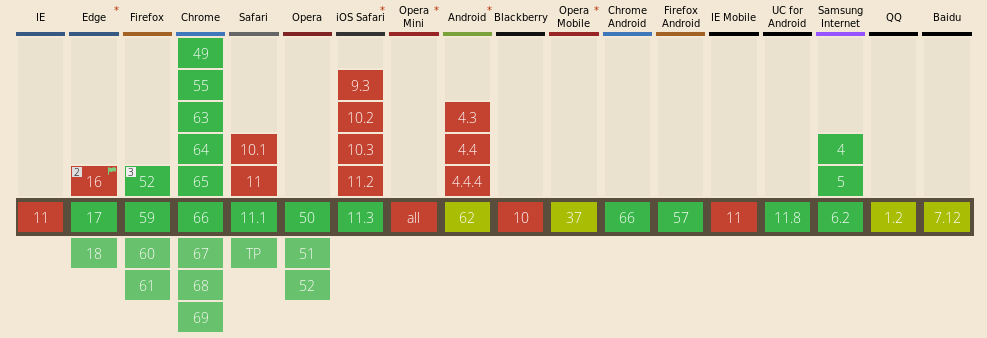
\includegraphics[width=1\textwidth]{ServiceWorker_all}
	\grayRule
	\caption[Browserkompatibilität für Service Worker]{Browserkompatibilität für Service Worker, Quelle: ~\cite{caniuse-sw}}
	\label{fig:serviceworker}
\end{figure}
%
Mit dem Service Worker können, wie mit dem App Cache, statische Ressourcen sofort beim ersten Besuch der Seite im Cache gespeichert werden. Es lässt sich hierbei unterscheiden, ob die Daten vor der ersten Verwendung, oder später im Cache gespeichert werden sollen. Für den ersten Fall eignen sich statische Inhalte wie Schriften oder JavaScript--Dateien, für den zweiten größere Ressourcen, die nicht sofort benötigt werden.\\
Zusätzlich bietet der Service Worker die Möglichkeit, auf Interaktionen zu reagieren. Den NutzerInnen kann angeboten werden, bestimmte Inhalte der Seite, wie zum Beispiel ein Video, später bzw. offline anzuschauen. Diese werden dann im Cache gespeichert und sind somit offline verfügbar.
Service Worker erlauben außerdem den Zugriff auf Push-Benachrichtigungen und das Background Sync \gls{API}. Die Hintergrundsynchronisation kann einmalig oder in festgelegten Intervallen stattfinden und ist besonders für nicht dringende Aktualisierungen wertvoll~\cite{offline_cookbook}.